% Spec C[x]: closed points (x-a) on a line, plus the generic point (0) above.
% Source: book/tex/alg-geom/spec-examples.tex (Spec C[x]).
\documentclass[border=2mm]{standalone}
\usepackage{amsmath}\usepackage{amssymb}\usepackage{tikz}
\begin{document}
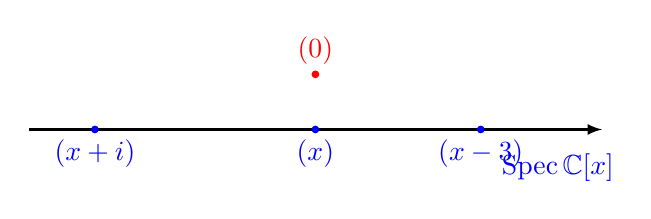
\begin{tikzpicture}[scale=0.7]
  \draw[thick,-latex] (-5.2,0) -- (5.2,0);
  \fill[blue] (0,0) circle (2pt) node[below] {$(x)$};
  \fill[blue] (3,0) circle (2pt) node[below] {$(x-3)$};
  \fill[blue] (-4,0) circle (2pt) node[below] {$(x+i)$};
  \fill[red] (0,1) circle (2pt) node[above] {$(0)$};
  \node[blue] at (4.4,-0.7) {$\operatorname{Spec}\mathbb{C}[x]$};
\end{tikzpicture}
\end{document}
